% !TEX program = xelatex

\documentclass[aspectratio=169]{beamer}
% Template: https://github.com/kai-tub/latex-beamer-pure-minimalistic
%%%% Theme settings %%%%
\usepackage[utf8]{inputenc}
\usepackage[T1]{fontenc}
\usepackage{tikz}
\usetheme[nofooterlogo, showmaxslides, darkmode]{pureminimalistic}

\graphicspath{ {./images/}{./logo/} }

% Logos
\renewcommand{\logotitle}{\includegraphics%
  [width=.05\linewidth]{logos/pydantify_without_text.png}}
\renewcommand{\logoheader}{\includegraphics%
  [width=.2\linewidth]{logos/pydantify_without_text.png}}
\renewcommand{\logofooter}{}

% Colors
% \definecolor{title}{RGB}{255, 255, 0} % Yellow
% \definecolor{title}{RGB}{172, 71, 189} % NetAutLabs
\definecolor{title}{RGB}{255, 255, 255}
\renewcommand{\beamertitlecolor}{title}

% Code
\usepackage{listings}
\usepackage{minted}
\usemintedstyle{rrt}

% Animation
\usepackage{animate}


% Notes
\setbeamertemplate{note page}{\pagecolor{yellow!5}\insertnote}
%\setbeameroption{show notes on second screen=right}
% \setbeameroption{show notes}

\title{Pydantify}
\subtitle{NetAutoberfest 2025}
\author{Urs Baumann}
% \institute{Swisscom}
\date{02.10.2025}

\begin{document}


{
% Set background image for the first page
% \setbeamertemplate{background}
% {
%   \includegraphics[height=\paperheight]{logos/pydantify_without_text.png}
% }
\frame{\titlepage}
}


\begin{frame}[fragile]
  \frametitle{Urs Baumann}

  \begin{minted}[fontsize=\small]{python}
>>> qr = QRCode()
>>> qr.add_data("https://www.linkedin.com/in/ubaumannch")
>>> qr.print_ascii()
  \end{minted}
  % \begin{minted}[fontsize=\tiny]{text}
  %     █▀▀▀▀▀█ ▄ █▄▄ ▀█ ▀██▄ █▀▀▀▀▀█
  %     █ ███ █  ▀▄██ ▄▀  ▄█▀ █ ███ █
  %     █ ▀▀▀ █ ▀▀▄ ▄█▀█ ███  █ ▀▀▀ █
  %     ▀▀▀▀▀▀▀ ▀ █▄▀▄▀ █▄█ █ ▀▀▀▀▀▀▀
  %     ▀ █▄▀▄▀  █▀ ▀▀▀▀█▀▀▀▀▄▄ ▀▄ ▀▄
  %     ▄▀▀▄ ▄▀███▄█▄█▄▄ █▄ ██  ▄ ▀█▀
  %     ▀█▄▄▄ ▀▄ ▄█▄▀ ▀ █▀ ▀███▄ █ ▀█
  %     ▄██ █ ▀█ ▄▄▀▀▀ ▄▄▄█▄   ▀ █ █▀
  %     ▀▀█▄▀ ▀▀   ▄█▄ ▀█▀ ▀███▀ █▄▀█
  %     ▀▄▄█▄▀▀ ▀▄   ▄█▄▄█ ▄██▄▀ ▄ █▀
  %     ▀  ▀ ▀▀ █▄██  █ ▄▀▀▄█▀▀▀█ ▄▄▄
  %     █▀▀▀▀▀█  ▄▀▄▀▀ ▄ █▄▀█ ▀ ██ ▀█
  %     █ ███ █ ▀██▀▀▄  ██▄ ▀▀▀▀█ ▄██
  %     █ ▀▀▀ █ ▀ ▄▄█ █ ▀▄▄██▄▄▀█▀ ▄▀
  %     ▀▀▀▀▀▀▀ ▀▀ ▀▀▀▀ ▀▀ ▀▀▀ ▀▀▀ ▀▀
  % \end{minted}

  \includegraphics[height = 0.6\textheight]{images/qrcode.png}

\end{frame}


\begin{frame}[fragile]
  \frametitle{CLI config vs NETCONF}

  \begin{columns}
        \column{.4\textwidth}
        \begin{minted}[
frame=none,
framesep=2mm,
baselinestretch=1.3,
fontsize=\tiny]{text}
sw04-pod-6(config)#int gi1/0/24
sw04-pod-6(config-if)#no switchdown
                                ^
% Invalid input detected at '^' marker.

sw04-pod-6(config-if)#

\end{minted}
        \column{.6\textwidth}
        \begin{minted}[
frame=none,
framesep=2mm,
baselinestretch=1.3,
fontsize=\tiny]{text}
<rpc-error>
  <error-type>application</error-type>
  <error-tag>invalid-value</error-tag>
  <error-severity>error</error-severity>
  <error-path xmlns:t="http://example.com/schema/1.2/config">
    /t:top/t:interface[t:name="Ethernet0/0"]/t:mtu
  </error-path>
  <error-message xml:lang="en">
    MTU value 25000 is not within range 256..9192
  </error-message>
</rpc-error>
\end{minted}
    \end{columns}

    
\end{frame}

\begin{frame}[fragile]
  \frametitle{How do engineers work with YANG?}
  \begin{minted}[
frame=lines,
framesep=2mm,
baselinestretch=1.3,
fontsize=\tiny,
linenos]{django}
<config>
<if:interfaces xmlns:if="urn:ietf:params:xml:ns:yang:ietf-interfaces">

  <if:interface>
    <if:name>Vlanif{{ interface.name }}</if:name>
    <if:description>uplink</if:description>
    <if:type xmlns:iana-if-type="urn:ietf:params:xml:ns:yang:iana-if-type">iana-if-type:propVirtual</if:type>
    <ip:ipv4 xmlns:ip="urn:ietf:params:xml:ns:yang:ietf-ip">
      <ip:address>
        <ip:ip>{{ interface.ip.split("/")[0] }}</ip:ip>
        <ip:prefix-length>{{ interface.ip.split("/")[1] }}</ip:prefix-length>
      </ip:address>
    </ip:ipv4>
  </if:interface>

</if:interfaces>
</config>
\end{minted}
\end{frame}

\begin{frame}{What I want \texttt{I}}
\centering
\animategraphics[autoplay, autopause, height = 0.8\textheight]{5}{animated/pydantify_demo}{00}{69}
\end{frame}

\begin{frame}
  \frametitle{What I want \texttt{II}}
  \centering
  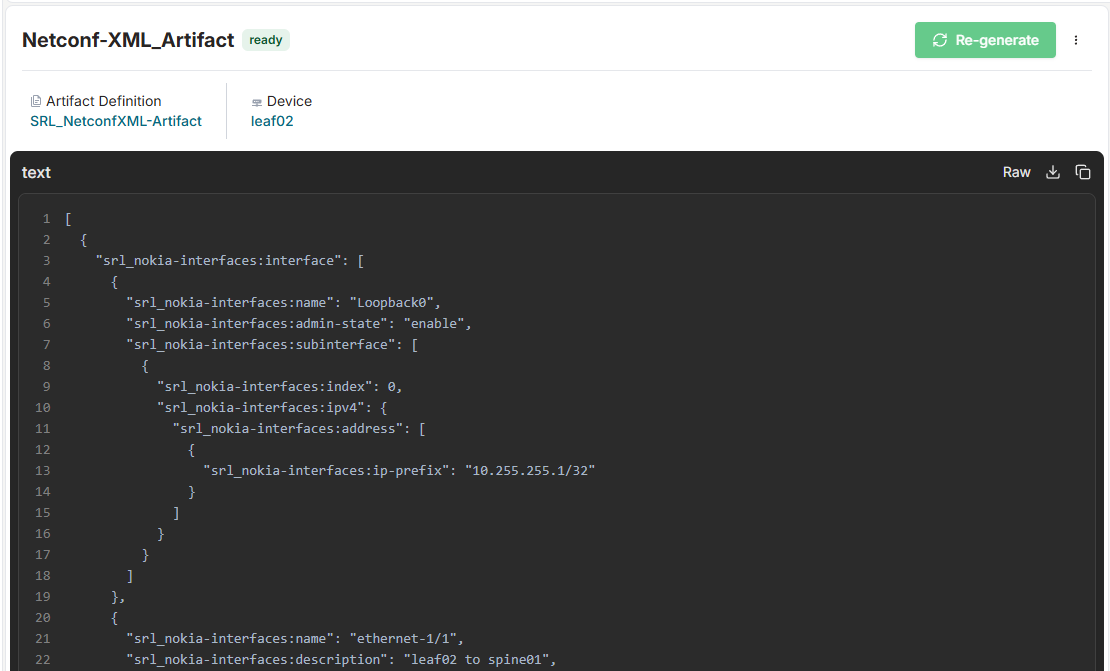
\includegraphics[height = 0.8\textheight]{images/netconf-xml-artifact.png}

\end{frame}

\begin{frame}
  \frametitle{What I want \texttt{III}}
  \begin{itemize}
    \setlength\itemsep{1em}
    \item Python objects with typing, validation and documentation
    \item Consumable / as intuitive and user-friendly as possible
    \item IDE autocompletion
    \item IDE error checks
    \item IDE type-hints
    \item Serialization / Deserialization
  \end{itemize}
\end{frame}


\begin{frame}
  \frametitle{Eco-System}
  \begin{itemize}
    \setlength\itemsep{1em}
    \item \href{https://github.com/robshakir/pyangbind}{pyangbind}
    \item \href{https://github.com/openconfig/ygot}{ygot}
    \item \href{https://github.com/CiscoDevNet/ydk-gen}{YANG Development Kit (ydk-gen)}
  \end{itemize}
\end{frame}


\begin{frame}
  \frametitle{How it started}
  \begin{itemize}
    \setlength\itemsep{1em}
    \item Midterm Project @ Eastern Switzerland University of Applied Sciences\\ Walther, Dominic and Jovicic, Dejan (2023)\\ \textbf{Make Model Driven Network Automation Pythonic}\\\url{https://eprints.ost.ch/id/eprint/1089/}
    % \item v0.5.0 Dec, 2022 \textemdash \ First public version
    % \item v0.6.0 Oct, 2024 \textemdash \ Use Pydantic v2 
    % \item v0.7.0 Jan, 2025 \textemdash \ Improve types like decimal64
    % \item v0.8.0 Feb, 2025 \textemdash \ Fix mandatory list keys
  \end{itemize}
\end{frame}

\begin{frame}
  \frametitle{Now}
  \begin{itemize}
    \setlength\itemsep{1em}
    \item \url{https://pydantify.github.io/pydantify/}
    \item \url{https://github.com/pydantify/pydantify}
    \item \url{https://pypistats.org/packages/pydantify}
  \end{itemize}
\end{frame}

\begin{frame}
  \frametitle{Vendor}
  \begin{itemize}
    \setlength\itemsep{1em}
    \item \url{https://github.com/srl-labs/pydantic-srlinux/}\\\textit{experimental project}
    \item \url{https://www.youtube.com/watch?v=CM3sT55zwt0}\\How can you use Pydantify? \textemdash \ Roman Dodin (Nokia)
  \end{itemize}
\end{frame}

{
\setbeamercolor{background canvas}{bg=black}
\begin{frame}[plain,c]
  \begin{center}
    \Huge \color[rgb]{1,1,1}Demo
  \end{center}
\end{frame}
}

\begin{frame}
  \frametitle{Challanges / not supported}
  \begin{itemize}
    \setlength\itemsep{1em}
    \item Pydantify: YANG > Pyyang > \textbf{JSONSchema} > DMGC > Pydantic
    \item Context-aware validation
    \item must / if / \dots
    \item xPath
    \item bits / decimal64 representation
    \item RegEx
  \end{itemize}
\end{frame}

{
\setbeamercolor{background canvas}{bg=black}
\begin{frame}[plain,c]
  \begin{center}
    \Huge \color[rgb]{1,1,1}Questions?
  \end{center}
\end{frame}
}
\end{document}